\documentclass{scrreprt}
\usepackage{listings}
\usepackage[]{graphicx}

\begin{document}

\chapter{The Idea of OmniView}
OmniView is planned to be an omniscient data-visualization and analysis tool. 
OmniView itself shouldn't need to know anything about any given data-producer at compile-time, but should still be able to visualize the produced information.
OmniView itself shouldn't need to know anythink about any given analysis-tool at compile-time, but should still be able to use an analysis-API. 
In order for OmniView to work this way, there shall be a structured architectural approach, to enable modular development.
This includes dataproducer devices as well as analysis-tools.

\begin{figure}
    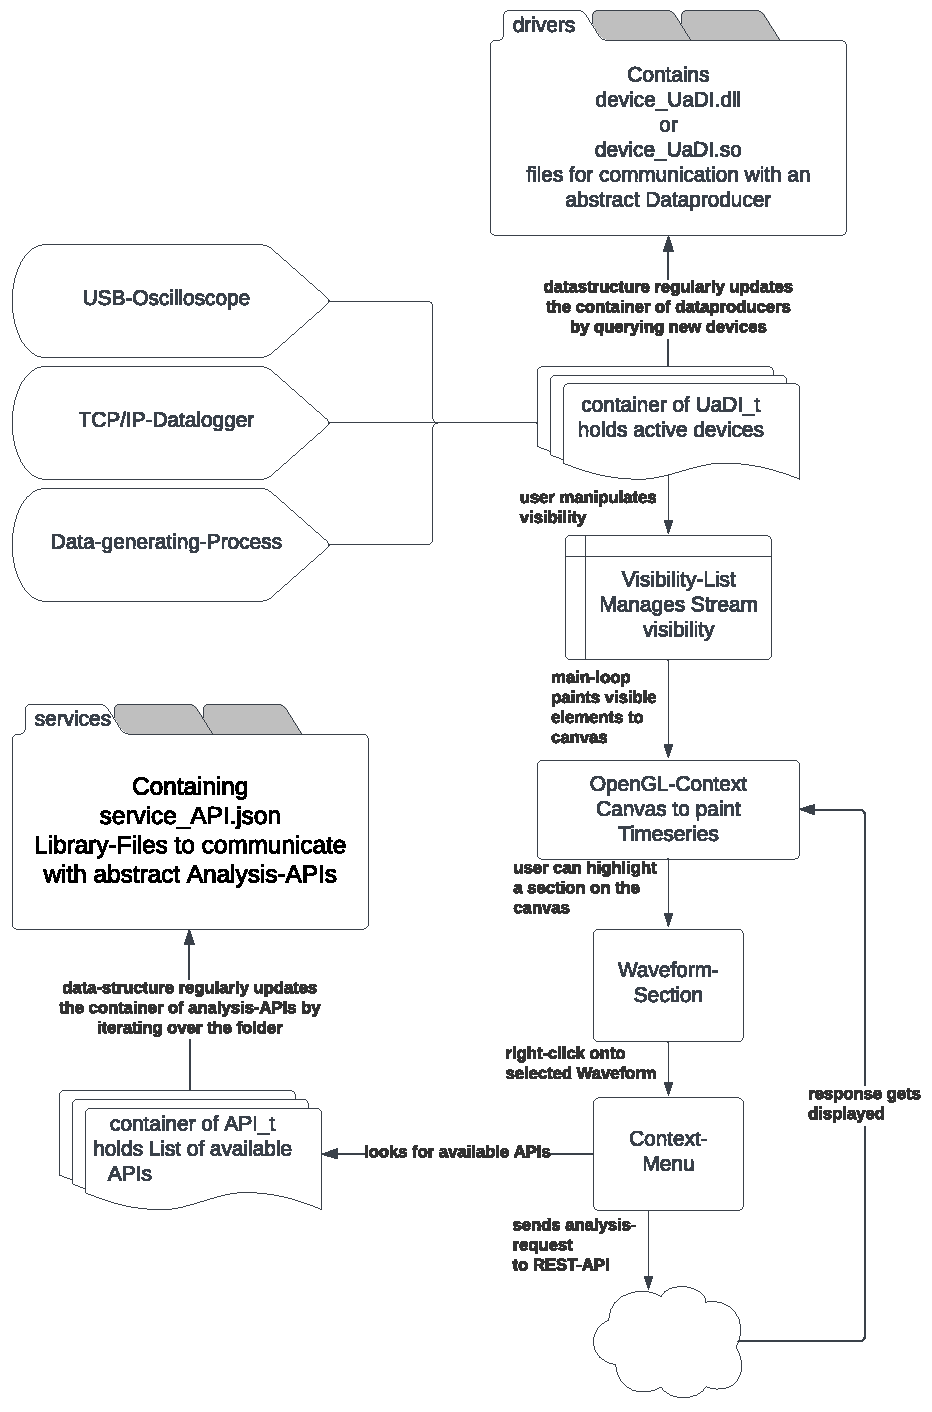
\includegraphics[width=.9\textwidth]{./assets/pictures/overview.pdf}
    \caption[]{Brief overview of the proposed structure}
    \label{fig:overview}
\end{figure}


There shall be a unified way to interact with an abstract data-producer.
This includes devices such as:
\begin{enumerate}
    \item a USB-oscilloscope
    \item a TCP/IP client, sending a continuous stream
    \item a USB-logic-analyzer
    \item a random-number-generator
    \item a filedescriptor
\end{enumerate}

Since it is not known at compile-time, which devices will be used at runtime, the code can't be linked statically into OmniView (or any other data-consumer for that matter). 
Therefor an interface shall be defined, that gets used by the consumer, but the implementation of the data-handling ought to be provided in a dynamically linked library. 
From here on forward we will refer to this as \lstinline|DLL| even though \lstinline|.dll| and \lstinline|.so| are meant equally. 
If a windows \lstinline|.dll| or a linux \lstinline|.so| is meant specifically, please use the terms \lstinline|.dll| or \lstinline|.so|, otherwise \lstinline|DLL|. 
Be aware, that this \lstinline|DLL| does not necessarily constitue an aquivalent to an actual device-driver with a communication-channel to the systems kernel.
\\
It appears, that all dataproducers that are relevant for OmniView can be abstracted in a certain way, and thus share the same function-calls in a \lstinline|DLL|.
There are three requirements:
\begin{itemize}
    \item Grabbing the next part of the data-stream asynchronusly
    \item The data-producer providing meta-information about itself 
    \item Send control-data from the consumer to the data-producer
\end{itemize}
This interprocess-communication comes with some additional hurdles.

\section{Memory Management Ideology}
Not only does OmniView not know about which devices will be connected at runtime, it also does neither know about the amount of devices that will be attached, nor does it know what data-rate the producers will provide.
Due to this uncertainties, a strongly structured memory allocation ideology needs to be implemented in order to minimize error-prone sections in the applications code.


\section[UaDI]{Unified abstract Data\-producer Interface}
The \textit{Unified abstract Data\-producer Interface} is the protocol that specifies the interprocess\-communication between the con\-sumer and the device, using the \lstinline|DLL|. 

\begin{figure}
    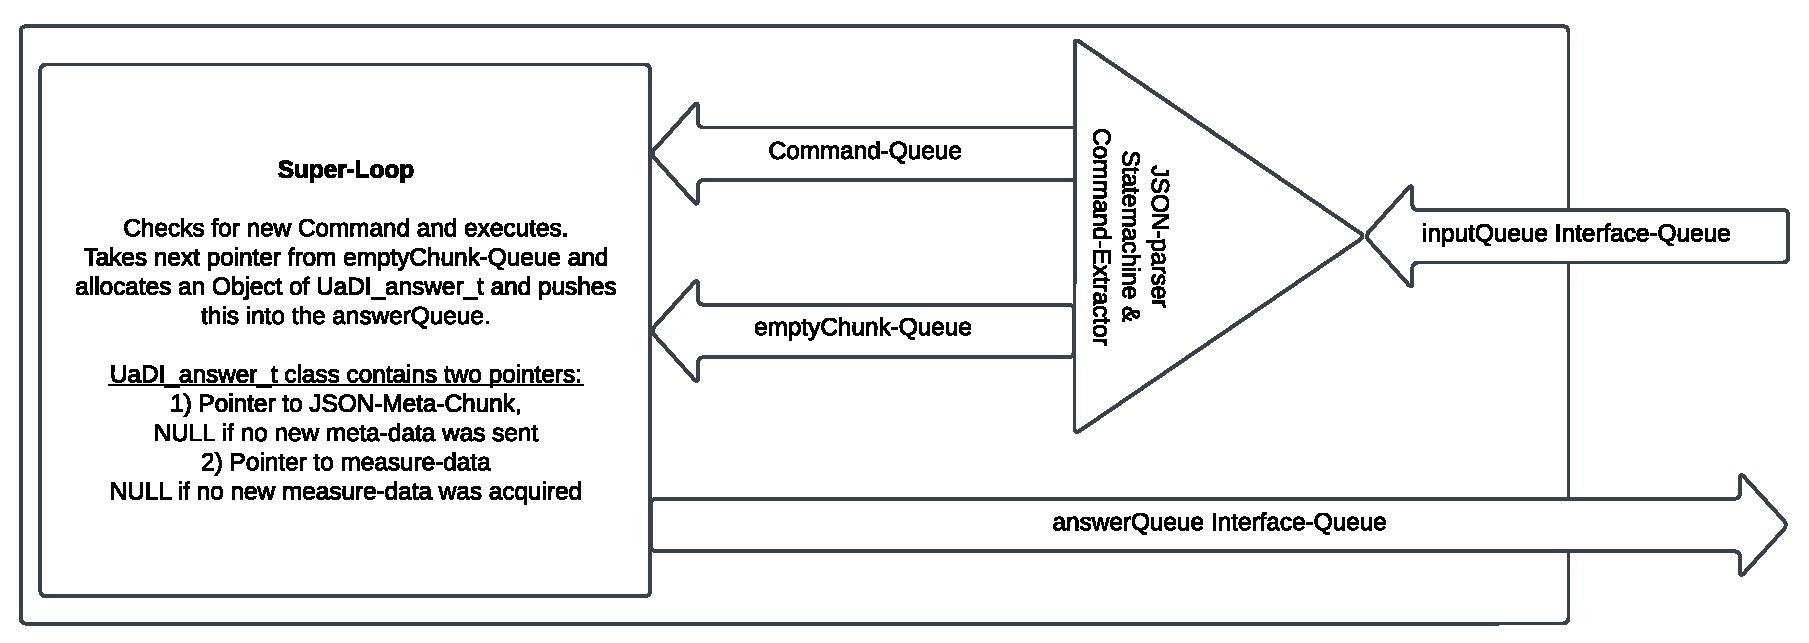
\includegraphics[width=.9\textwidth]{./assets/pictures/interface.pdf}
    \caption[]{Coarse structure of the DLL-interface}
    \label{fig:dllinterface}
\end{figure}





\chapter[Further Devl]{Further Development of OmniView}
OmniView as it is right now has a limited shelf-life. 
The current version will be deprecated somewhere around summer of 2024.
It will be replaced by a more modular approach, that consists of two separate pieces, called OmniDaemon and OmniView 2.0.
OmniView 2.0 will be written in Angular.
OmniDaemon will still be written in C++ and use the same approach for data-acquisition. 
The interprocess-communication between the data and the view on the data will be implemented by using websockets for live-streaming, REST for settings and downloading whole files and MQTT-Publishing for sending out alarms and similar fire-and-forget messages. 




\end{document}